\documentclass[11pt]{article}
\usepackage{fullpage,url}
\usepackage{amsmath,amsthm,amssymb}
\usepackage{graphicx}
\usepackage{eso-pic}
\usepackage{bm}
\usepackage{caption}
\usepackage{picins}   
\usepackage{microtype}
\usepackage{url}
\usepackage{enumerate}
\usepackage{pdfpages}
\usepackage[boxed,vlined]{algorithm2e}
\usepackage{nomencl}
\usepackage[letterpaper,top=1in,bottom=1in,left=1in,right=1in,nohead]{geometry}

\newcommand{\PhiB}{\mathbf{\Phi}}
\newcommand{\Ll}{\mathcal{L}}
\newcommand{\Nn}{\mathcal{N}}
\newcommand{\Uu}{\mathcal{U}}
\newcommand{\Ee}{\mathcal{E}}
\newcommand{\Aa}{\mathcal{A}}
\newcommand{\Hh}{\mathcal{H}}
\newcommand{\Ii}{\mathcal{I}}
\newcommand{\Ff}{\mathcal{F}}
\newcommand{\Vv}{\mathcal{V}}
\newcommand{\Tt}{\mathcal{T}}
\newcommand{\Pp}{\mathcal{P}}
\newcommand{\Ss}{\mathcal{S}}
\newcommand{\Cc}{\mathcal{C}}
\newcommand{\Oo}{\mathcal{O}}
\newcommand{\Bb}{\mathcal{B}}
\newcommand{\Rr}{\mathcal{R}}
\newcommand{\Rm}{\mathrm{R}}
\newcommand{\CB}{\mathbf{C}}
\newcommand{\RB}{\mathbf{R}}
\newcommand{\xB}{\mathbf{x}}
\newcommand{\yB}{\mathbf{y}}
\newcommand{\XB}{\mathbf{X}}
\newcommand{\YB}{\mathbf{Y}}
\newcommand{\fB}{\mathbf{f}}
\newcommand{\ZB}{\mathbf{Z}}
\newcommand{\SB}{\mathbf{S}}
\newcommand{\AB}{\mathbf{A}}
\newcommand{\WB}{\mathbf{W}}
\newcommand{\EB}{\mathbf{E}}
\newcommand{\PB}{\mathbf{P}}
\newcommand{\BB}{\mathbf{B}}

\newcommand{\omitme}[1]{}
\newtheorem*{lemma}{Lemma}
\newtheorem{case}{Case}

\makeatletter
\newcommand{\specialnumber}[1]{%
  \def\tagform@##1{\maketag@@@{(\ignorespaces##1\unskip\@@italiccorr#1)}}%
}

\setlength{\parindent}{0in}
\setlength{\parskip}{6pt}

\DeclareMathOperator{\E}{E}
\DeclareMathOperator{\Var}{Var}
\DeclareMathOperator{\Unif}{Unif}
\newcommand{\argmin}{\operatornamewithlimits{argmin}}

\title{Face Index Map Generation}

\author{Prateep Mukherjee, Shireen Elhabian and Ross Whitaker}

\begin{document}
\maketitle
\makenomenclature
%\vspace{-10pt}
\section{Method}
%\vspace{-20pt}

 \subsection{Introduction} 
%\vspace{-10pt} 
 Shape analysis in medical imaging involves analyzing shapes and properties of anatomical parts of individual patients as well as over a large population. Thus, statistical shape modeling can be classified into two groups. First, when the only input to the system is a binary segmented volume with every voxel labeled [0,1], statistical analysis involves modeling the variations of postional data. Hence, this is called \textbf{positional} analysis. The second group is more general, where every individual voxel is associated with certain significant \emph{attributes}, like thickness, scalar field, tensile strength etc. These attributes provide clinical information regarding stucture and morphology. Therefore, such a model is called \textbf{functional} analysis, since the image data is a function of certain attributes. Functional shape analysis evidently provides better and accurate medical treatment, as it jointly models the variations in shape as well as anatomical features of shape. 

 \subsection{Goal} 
%\vspace{-10pt} 
 The aim of this method is to generate a feature volume($F$), within a narrow-band, given an image domain($\Omega$) and a surface($M$). $M$ is parametrized by a set of vertices($\Vv$) and faces($\Ff$). Each vertex $v \in \Vv$  is associated with $d$ attribute values($\mathcal{S} : \Re \rightarrow \Re^{d}$). The nearest vertex($v^{*}$) to a voxel is mathematically defined as follows:
  \begin{eqnarray*}
		   &v^{*} = \argmin\limits_{v \in \mathcal{V}} \; (d_{\bar{x}',v}), \; \; \forall \bar{x}' \in \mathcal{N} \\
          \mathcal{N} :& \left\{ \bar{x} \; |
         				  \left\{ \begin{array}{cc}
		                   1, & \mbox{$-k \le (\bar{x} - \bar{v}) \le k$} \\
        				   0, & otherwise
         \end{array} \right\} , \forall (\bar{x},\bar{v}) \in \Omega
         \right\}
  \end{eqnarray*}
 
 Here, $\mathcal{N}$ denotes the narrow-band, and $d_{\bar{x},v}$ denotes the \emph{barycentric distance} for voxel $\bar{x}$ to vertex $v$. Therefore, the feature volume $F$, at each voxel, is simply defined as the feature attribute of its nearest face. That is,
 \vspace{-5pt}
\begin{equation}
   F(\bar{x}) = \mathcal{S}(v^{*}), \; \; \; \; \forall \bar{x} \in \Omega, v^{*} \in \mathcal{V}
 \label{eq1}
\end{equation}

\printnomenclature
\nomenclature{$F$}{feature volume}%
\nomenclature{$\Omega$}{image domain($\Re^3$)}%
\nomenclature{$M$}{surface mesh}%
\nomenclature{$\Vv$}{vertices $\in M$}%
\nomenclature{$\Ff$}{faces $\in M$}%
\nomenclature{$\mathcal{N}$}{narrow-band $\in \Omega$}%
\nomenclature{$\mathcal{S}$}{set of attributes for each vertex}%

 \subsection{KD-tree} 
% \vspace{-10pt}
 The easiest approach to solve this is to use k-nearest neighbor(kNN) metric. KD-trees\cite{KD} are often used to get nearest neighbors for a point in k-dimensional space. KD-trees recursively split the domain $\Omega$ in two parts, and searches over each half in order to get the nearest points. This divide and conquer approach provides $O(\log n)$ query time, which  is a major improvement over linear search in real-time applications. 
 
 \subsection{Potential problems} 
%\vspace{-10pt} 
 However, KD-trees do not have a prior knowledge of the topology. This fails to find accurately the triangle with minimum barycentric distance(Fig \ref{fig1}a). To solve this problem, we generate a list of candidate face indices within a radius($R$), for every voxel($v$). The winning face is selected from this list, which has the minimum distance from $v$. Each voxel is divided into a number of sub-voxels, and for every sub-voxel a candidate face is selected. This provides a set of candidate faces for every voxel. The flowchart for this method is described in Algorithm \ref{alg1}.
 
 \subsection{Choosing the search diameter} 
% \vspace{-10pt}
 The maximum radius of search for a voxel is computed based on its distance to the isosurface($\S==igma$), the number of sub-voxels($h$) and the maximum edge-length($s$) of all faces($\mathcal{F}$). This is illustrated in Fig. \ref{fig1}b. In fig. \ref{fig1}b, $q$ is the physical distance from the center of the voxel($M$) to its corner: $q \sim h \times \sqrt{3}$. $l_\delta$ for a triangle is approximately equal to $\frac{s}{\sqrt{3}}$, assuming an equilateral $\triangle$. Also, $\triangle$ MVC, formed by the center of the voxel(M), centroid of a face(C) and one of its corner vertex(V), is a right-angled triangle. Therefore, using Pythagoras' theorem, the distance from M to V is $\sqrt{{l_\delta}^2 + \Sigma^2}$. Therefore, the maximum search radius $B = q + (\sqrt{{l_\delta}^2 + \Sigma^2})$.

\begin{figure}[hbt]
\begin{center}
 \[ \begin{array}{ccc}
 
  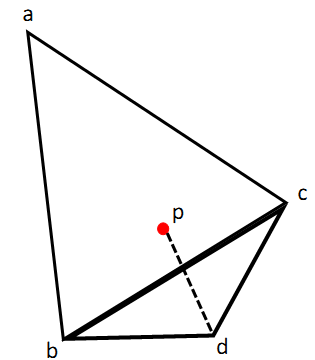
\includegraphics[scale=0.5]{fids_1.png} &
  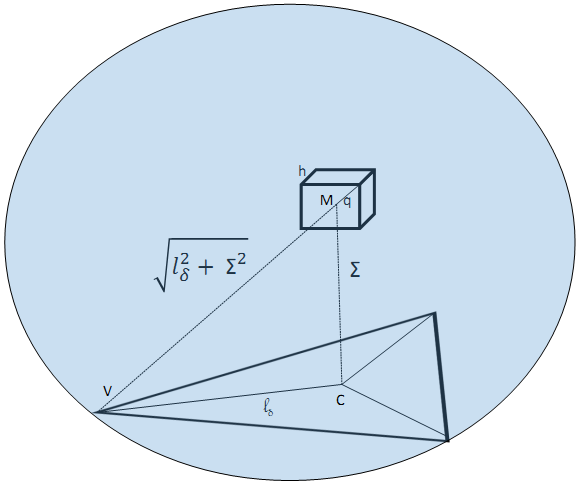
\includegraphics[scale=0.4]{fids_3.png} &
  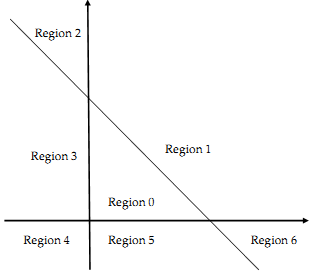
\includegraphics[scale=0.6]{fids_2.png} \\
  (a) & (b) & (c) \\
 \end{array} \]
\end{center}
\vspace{-20pt}
  \caption{{\bf(a)} Bad case for KD-tree. Point p is nearest to vertex(d), while it lies inside $\triangle$(abc); {\bf(b)} Illustrates the computation of the search radius; {\bf(c)} Partitioning the $\alpha\beta$-plane by triangle domain}
  \label{fig1}
\end{figure}

 \subsection{Barycentric Distance from Point to $\triangle$} 
% \vspace{-10pt}
 The problem is to compute the minimum distance between a point $\PB$ and a triangle $\triangle(\alpha,\beta) = \alpha \BB + \beta \EB_0 + (1-\alpha-\beta) \EB_1$, for $\alpha, \beta \{ \alpha, \beta : \alpha \in [0,1], \beta \in [0,1], \alpha + \beta \le 1 \}$. The minimum distance is computed by locating the values $(\bar{\alpha}, \bar{\beta})$ corresponding to the point on the triangle closest to $\PB$. \cite{PT}
 
\par The squared-distance function for any point on the triangle to $\mathbf{P}$ is $Q(\alpha,\beta) = |\triangle(\alpha,\beta) - \PB |^2$. Expanding the quadratic term, $Q(\alpha,\beta)$ can be written as:

\begin{equation}
  Q(\alpha,\beta) = a \alpha^2 + 2b\alpha\beta + c\beta^2 + 2d\alpha + 2e\beta + f
  \label{eq2}
\end{equation}
where, $a = \EB_0 \cdot \EB_0$, $b = \EB_0 \cdot \EB_1$, $c = \EB_1 \cdot \EB_1$, $d = \EB_0 \cdot (\BB - \PB)$, $e = \EB_1 \cdot (\BB - \PB)$ and $f = (\BB - \PB) \cdot (\BB - \PB)$.
 
The optimal values $\bar{\alpha},\bar{\beta}$ are obtained using calculus of variations on $Q$. The gradients are $\nabla_\alpha Q = 2(a\alpha + b\beta + d)$, and $\nabla_\beta Q =  2(b\alpha + c\beta + e)$. To solve eq. \ref{eq2}, we divide the $\alpha\beta$ plane into 7 regions(Fig. \ref{fig1}c). 

\par Suppose $(\bar{\alpha},\bar{\beta})$ is in region 1. The level curves of $Q$ are those curves in the $\alpha\beta$-plane for which $Q$ is a constant. The graph of $Q$ is a paraboloid. Hence, the level curves are ellipses. At the point where $\nabla Q = (0,0)$, the level curve degenerates to a single point $(\bar{\alpha},\bar{\beta})$, which is the global minimum. As the iso-values increase from here, the corresponding ellipses increase further away from $(\bar{\alpha},\bar{\beta})$. There is a smallest iso-value $V_0$ for which the corresponding ellipse just touches the triangle domain edge $\alpha+\beta=1$ at a value $\alpha = \alpha_0, \beta = 1 - \alpha_0$. For isovalues $V < V_0$, the corresponding ellipses do not intersect the triangle domain. For level values $V > V_0$, portions of the triangle domain lie inside the corresponding ellipses. In particular any points of intersection of such an ellipse with the edge must have a level value $V > V_0$. Therefore, $Q(\alpha, 1-\alpha) > Q(\alpha_0,\beta_0)$, for $\alpha \in [0,1]$, and $\alpha \neq \alpha_0$. The point $\alpha_0,\beta_0$ provides the minimum squared distance between $\PB$ and the triangle. 
 

\section{Algorithm}
\vspace{-10pt}
Following is a pseudo-code of the algorithm.
\vspace{-10pt}

\begin{algorithm}[H]
\caption{getFaceIndexList}
\dontprintsemicolon
\KwData{Narrow Band($N_B$), original volume($I$), Mesh($M$), $s_v$, $S_v$}
\KwResult{Map containing face indices for $I$}
\SetKwData{Output}{Output}
\SetKwData{Dist}{d}\SetKwData{Point}{p}\SetKwData{Thresh}{Thresh}
\SetKwData{fid}{faceId}
\SetKwData{candidates}{candidates}
\SetKwFunction{indexToPhysicalCoord}{indexToPhysicalCoord}
\SetKwFunction{physicalCoordToIndex}{physicalCoordToIndex}
\SetKwFunction{PointTriangleDistance}{PointTriangleDistance}
initialize \Output to be same size as $N_B$ \;
declare \candidates \tcc{a map to store all candiate faces for every super-voxel} 
initialize \Thresh \;
$I_\downarrow$ $\leftarrow$ downscale(I) \;
$I_\uparrow$ $\leftarrow$ upscale(I) \;
%get spacing and size of $I_\downarrow$ \;

\For{each voxel $v$ in $I_\downarrow$}{
  \Point $\leftarrow$ \indexToPhysicalCoord($v$) \;
  \For{each face $f$ in $M$}{
        \Dist $\leftarrow$ \PointTriangleDistance(\Point,$f$) \;
         \If{\Dist $\le$ \Thresh}{
                \candidates[$v$] $\leftarrow$ $f$ \;
         }
  }
}
\SetKwData{fidsMap}{faceIndexMap}
declare \fidsMap  \; \tcc{a map to store all faces for every voxel}
\For{each voxel $v$ in $N_B$}{
         $\Point_\uparrow$ $\leftarrow$ \indexToPhysicalCoord($v$) \;
	  $\Point_\downarrow$ $\leftarrow$ get position of $\Point_\uparrow$ in $I_\downarrow$ \;
	  $v_\downarrow$ $\leftarrow$ \physicalCoordToIndex($\Point_\downarrow$) \;
         \fid $\leftarrow$ \PointTriangleDistance($\Point_\downarrow$, \candidates[$v_\downarrow$] ) \; 
	  \Output[$v$] $\leftarrow$ \fid \;
	  \Point $\leftarrow$ get position of  $v$ in $I$ \;
	  $V$ $\leftarrow$ \physicalCoordToIndex(\Point) \;
	  \fidsMap[$V$] $\leftarrow$ \fid \;
}
\label{alg1}
\end{algorithm}

\section{Results}


\begin{figure}
 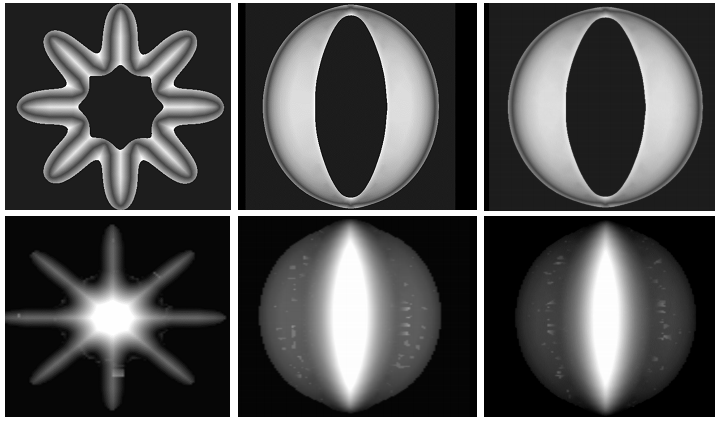
\includegraphics[width=\linewidth]{fids_4.png}
 \caption{Distance map generated using our method({\bf Top}), and KD-tree({\bf Bottom}). }
 \label{fig2}
\end{figure}

Distance maps generated from our method and that using KD-trees are shown in Fig.\ref{fig2}. It can be seen that distance transforms generated using our method is continuous and smooth, while that using KD-trees are more irregular.

\begin{thebibliography}{9}
\bibliographystyle{IEEbib}
\small
\addtolength{\itemsep}{-9pt}

\bibitem{KD}
John Louis Bentley, `Multidimensional binary search trees used for associative searching,' 
\emph{Commun. ACM}, 18(9):509-517, 1975.

\bibitem{PT}
David Eberly, `Distance Between Point and Triangle in 3D,'
\emph{Geometric Tools, LLC}, 2008.


\end{thebibliography}


\end{document}
